\documentclass[a4paper]{article}

\usepackage{INTERSPEECH2021}
\usepackage{booktabs}
\usepackage{graphicx}

% Align floats on a float page to the top instead of vertically centered
\makeatletter
\setlength{\@fptop}{0pt}
\makeatother

\title{NLU course project: Intent Classification and Slot Filling}
\name{Elena Deidda (mat. 267887)}

\address{
  University of Trento}
\email{elena.deidda@studenti.unitn.it}

\begin{document}

\maketitle

\section{Introduction}
This project compares two strategies for joint intent classification and
slot filling on ATIS, evaluated with Intent Accuracy and chunk-level Slot F1
(CoNLL): training a Transformer \emph{from scratch} (Part~A) versus
fine-tuning pre-trained encoders and decoders (Part~B). For Part~A, a
GPT-2-style decoder-only Transformer is the chosen architecture, with a
greedy hyper-parameter search performed over learning rate, architecture,
and dropout. For Part~B, pre-trained BERT~\cite{devlin2019} and
GPT-2~\cite{radford2019} are used, adapting the sub-tokenization strategy of
Chen et al.~\cite{chen2019} for slot label alignment. The best model overall
is BERT-base, reaching test Slot F1 0.955 and Intent Accuracy 0.975, against
0.888 and 0.934 for the best from-scratch model: pre-trained bidirectional
representations give a clear advantage on both tasks.

\section{Implementation details}
The backbone architectures (GPT-2 from scratch and the fine-tuning setup)
follow the course lab; the contributions below are original to this work.

\textbf{CLS placement (Part A).} Since the model is causal, the \texttt{CLS}
token is appended at the \emph{end} of each utterance rather than at the
start. The last position is the only one that has attended to the full
sequence, so its hidden state is used for intent classification; slot
decoding excludes this extra position before scoring with CoNLL.

\textbf{Per-architecture intent representation (Part B).} BERT uses the
\texttt{[CLS]} hidden state at position 0. GPT-2 is causal, so intent
classification instead uses the hidden state at the last \emph{real} token,
retrieved via the per-sequence length rather than the last padded position.

\textbf{Sub-token label alignment (Part B).} Following the strategy
discussed in~\cite{chen2019}, only the first sub-token of each word carries
the true slot label; remaining sub-tokens and special tokens are excluded
from the slot loss via \texttt{ignore\_index}. This reference is used as
conceptual guidance for the alignment rule, not as a code source.

\textbf{Multi-seed greedy search.} Each candidate in the greedy
hyper-parameter search (learning rate first, then architecture, then
dropout) is run over multiple seeds \emph{before} being compared to the
incumbent, rather than only the final model. This reduces the risk of
selecting a configuration that owes its apparent advantage to a favorable
seed instead of a real effect of the hyper-parameter.

\section{Results}
All models are evaluated on the test set over multiple seeds (mean$\pm$std);
hyper-parameters are selected on the \emph{dev} Slot F1 to avoid test-set
leakage. Table~\ref{tab:nlua} and Figure~\ref{fig:nlua} report Part~A: the
learning-rate search already reaches most of the achievable performance, and
only \texttt{n\_heads} contributes a further, modest gain -- every other
architecture candidate falls below the incumbent and is discarded. Table~\ref{tab:nlub}
reports Part~B: BERT clearly outperforms GPT-2 on slot filling (0.955 vs.\
0.915 test F1), consistent with BERT's bidirectional context being better
suited to per-token tagging than GPT-2's left-to-right attention. Scaling to
the large/medium variant does not improve test metrics for either family
despite 3$\times$ more parameters, suggesting ATIS is already saturated by
base-sized pre-trained models. Figure~\ref{fig:params} makes this explicit:
moving from a from-scratch model to a pre-trained one yields a large jump in
Slot F1, while further scaling within Part~B yields essentially none.

\textbf{Error analysis.} Beyond aggregate scores, Figure~\ref{fig:perslot}
breaks down test Slot F1 by slot type for the two best fine-tuned models. On
the most frequent slots both are strong, but BERT's advantage widens precisely
on slots whose interpretation depends on context from \emph{both} sides --
\texttt{airline\_name} (0.99 vs.\ 0.86), \texttt{depart\_time.period\_of\_day},
\texttt{aircraft\_code}, \texttt{class\_type} -- confirming that bidirectional
attention, not scale, drives the gap, since GPT-2-medium already has 3$\times$
BERT-base's parameters. The hardest slot for both is the generic
\texttt{city\_name} (F1 0.64/0.55), routinely confused with the directional
\texttt{fromloc}/\texttt{toloc.city\_name}. Intent classification is by contrast
nearly solved: the best BERT misclassifies only 23 of 893 test utterances, and
the residual errors (Figure~\ref{fig:intentcm}) are dominated by compound
intents such as \texttt{flight+airfare} collapsing onto their majority
component \texttt{flight}, rather than genuine semantic confusions.

\begin{table}[t]
  \centering
  \caption{Part~A --- best model per step (231K param. throughout). Final:
           $d{=}64$, 4 heads, 2 layers, FFN 256, dropout 0.}
  \label{tab:nlua}
  \begingroup
  \footnotesize
  \setlength{\tabcolsep}{3pt}
  \begin{tabular}{llrrr}
    \toprule
    Step & Adopted & Dev F1 & Test Slot F1 & Test Int.\ Acc \\
    \midrule
    0 -- lr           & $0.01$    & 0.929 & 0.876$\pm$0.007 & 0.921$\pm$0.017 \\
    1 -- architecture & heads$=$4 & \textbf{0.941} & \textbf{0.888$\pm$0.006} & \textbf{0.934$\pm$0.006} \\
    2 -- dropout      & none (0)  & 0.941 & 0.888$\pm$0.006 & 0.934$\pm$0.006 \\
    \bottomrule
  \end{tabular}
  \endgroup
\end{table}

\begin{figure}[t]
  \centering
  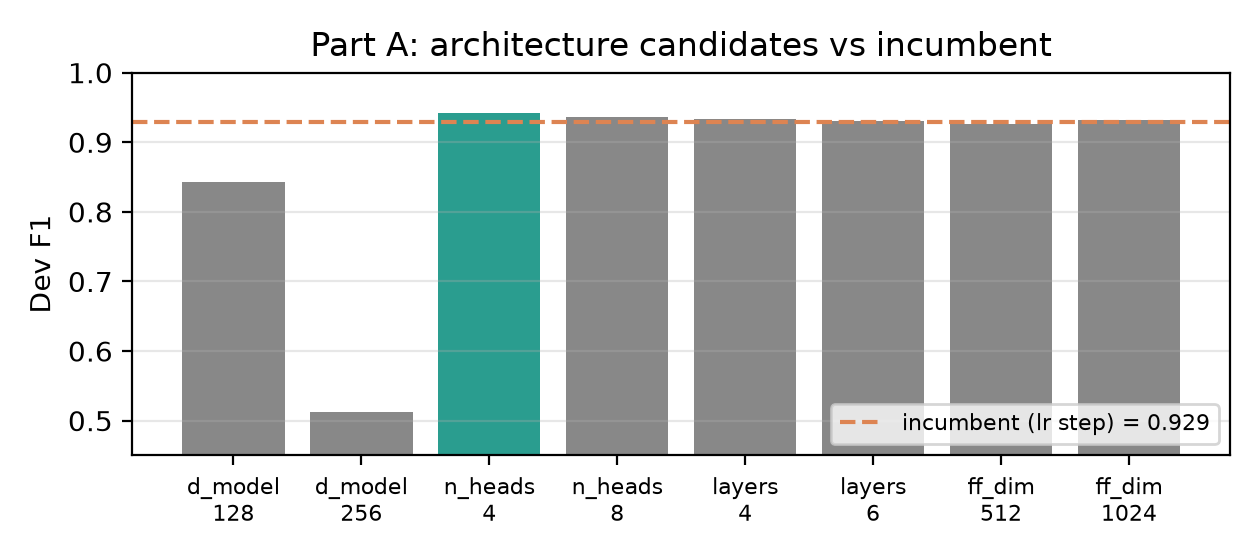
\includegraphics[width=\linewidth]{nlu_partA_architecture.png}
  \caption{Part~A: dev F1 of every architecture candidate against the
           incumbent score (dashed line); only \texttt{n\_heads}$=$4 wins.}
  \label{fig:nlua}
\end{figure}

\begin{table}[t]
  \centering
  \caption{Part~B --- fine-tuning (best lr/dropout per family).}
  \label{tab:nlub}
  \begingroup
  \footnotesize
  \setlength{\tabcolsep}{3pt}
  \begin{tabular}{lrrrr}
    \toprule
    Model & Param & Dev F1 & Test Slot F1 & Test Int.\ Acc \\
    \midrule
    BERT-base    & 109.6M & \textbf{0.984} & \textbf{0.955$\pm$0.002} & \textbf{0.975$\pm$0.001} \\
    BERT-large   & 335.3M & 0.983 & 0.955$\pm$0.001 & 0.975$\pm$0.002 \\
    GPT-2-base   & 124.6M & 0.963 & 0.915$\pm$0.004 & 0.971$\pm$0.002 \\
    GPT-2-medium & 355.0M & 0.964 & 0.913$\pm$0.002 & 0.969$\pm$0.003 \\
    \bottomrule
  \end{tabular}
  \endgroup
\end{table}

\begin{figure}[t]
  \centering
  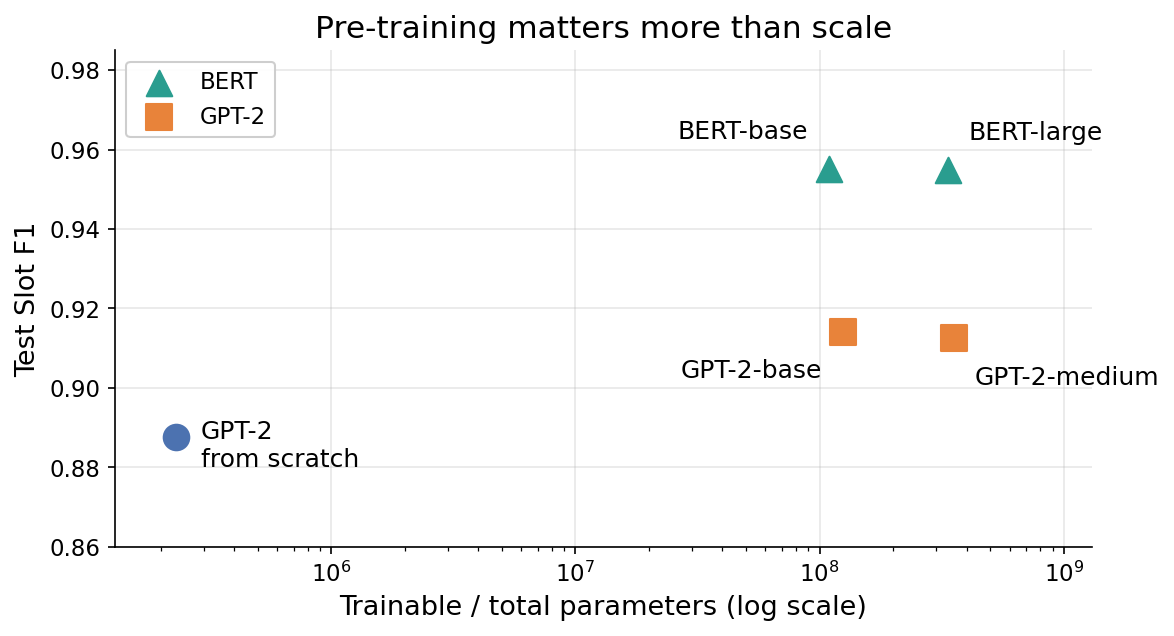
\includegraphics[width=\linewidth]{nlu_params_vs_f1.png}
  \caption{Test Slot F1 vs.\ parameter count (log scale): the jump from
           Part~A to Part~B dwarfs any gain from scaling within Part~B.}
  \label{fig:params}
\end{figure}

\begin{figure}[t]
  \centering
  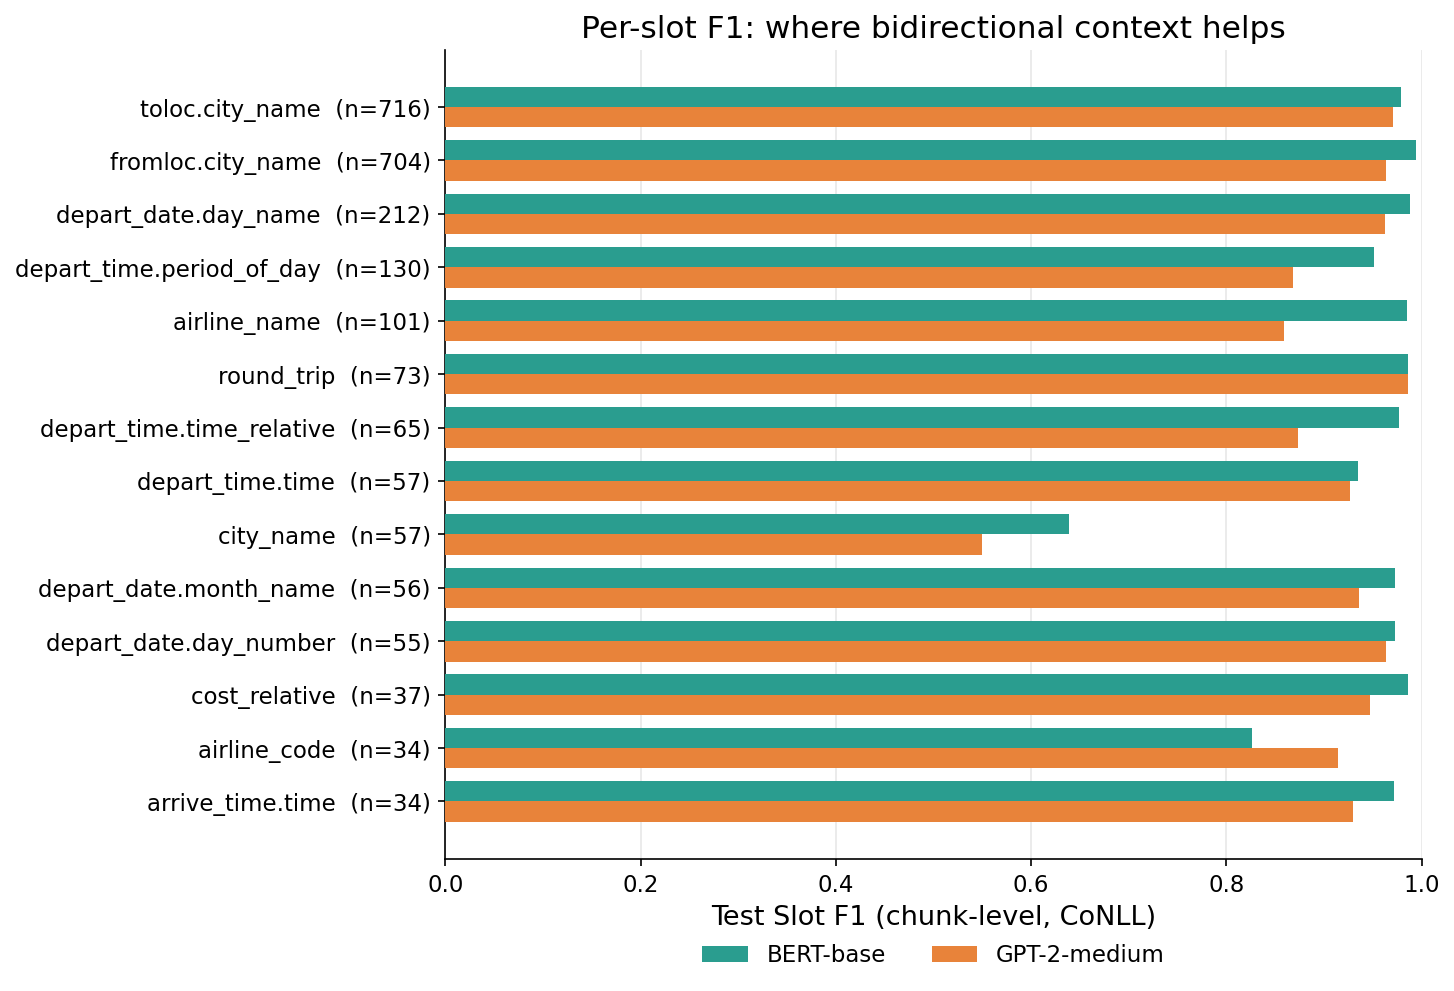
\includegraphics[width=\linewidth]{nlu_perslot_f1.png}
  \caption{Per-slot test Slot F1 (slots with support $\geq20$, $n$ = test
           occurrences): BERT vs.\ GPT-2-medium. The gap widens on
           context-dependent slots, not on the most frequent ones.}
  \label{fig:perslot}
\end{figure}

\begin{figure}[t]
  \centering
  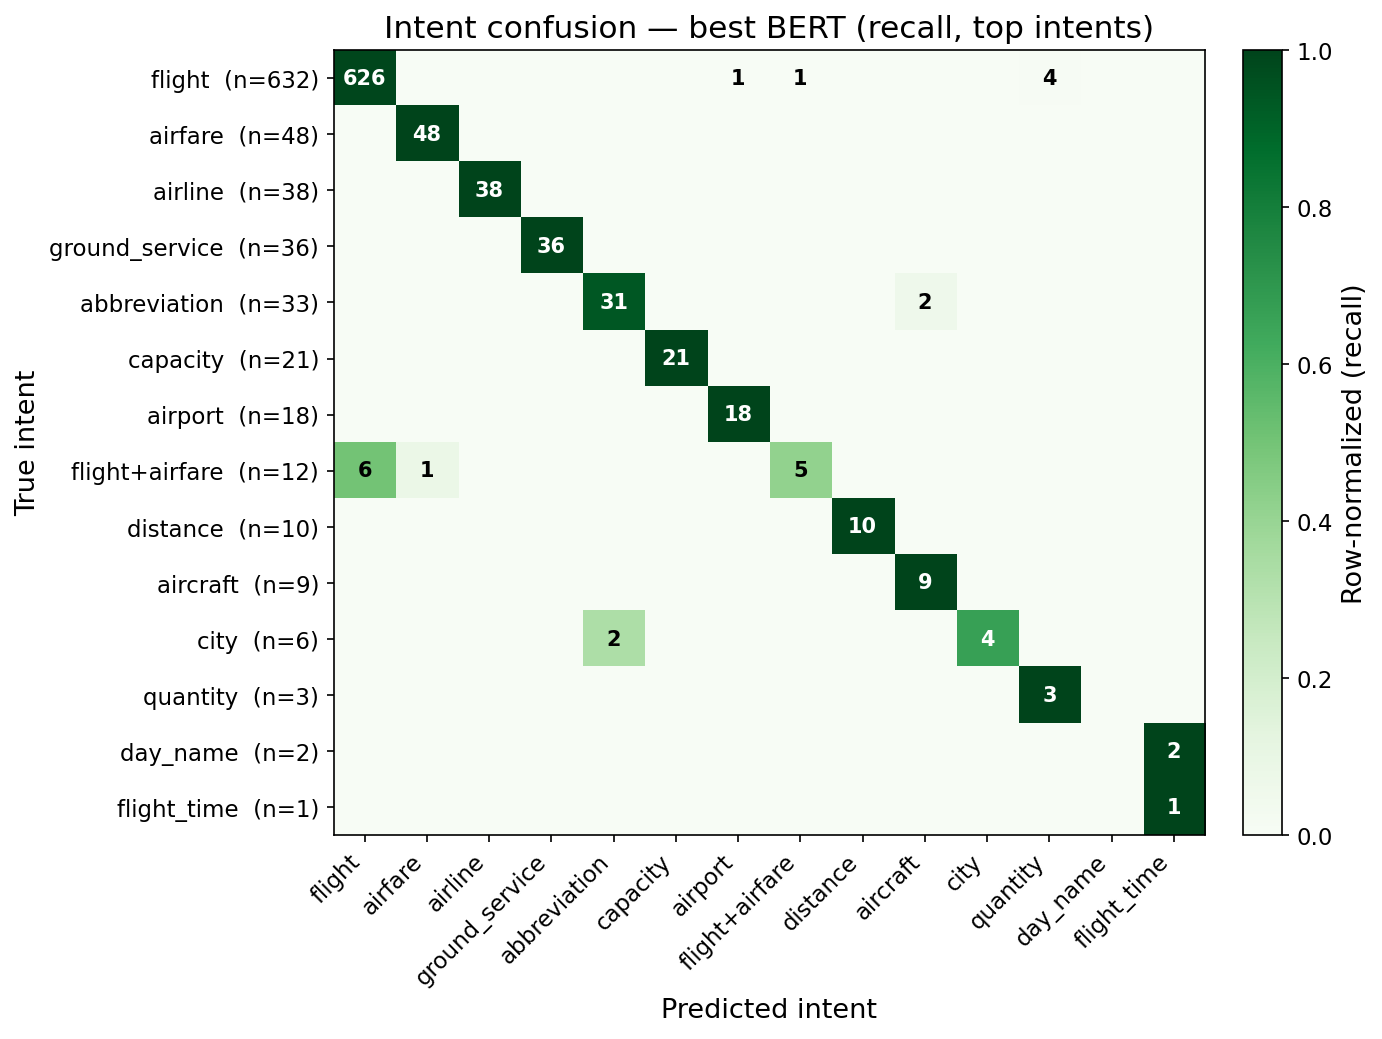
\includegraphics[width=\linewidth]{nlu_intent_confusion.png}
  \caption{Intent confusion (row-normalized recall) of the best BERT on the
           ATIS test set; cells show raw counts. Only 23/893 errors, mostly
           compound intents mapped to \texttt{flight}.}
  \label{fig:intentcm}
\end{figure}

\bibliographystyle{IEEEtran}
\bibliography{mybib}

\vspace{1mm}
\noindent{\footnotesize\textit{Declaration of AI use: a generative-AI assistant
(Claude, Anthropic) was used to help set up and debug the remote GPU training
environment, run the experiments, generate the figures, and edit the language
of this report. The choice of hyper-parameters to search, the model
architecture, and the interpretation of the results are the author's own.}}

\end{document}